%% bare_jrnl_compsoc.tex
%% V1.4b
%% 2015/08/26
%% by Michael Shell
%% See:
%% http://www.michaelshell.org/
%% for current contact information.
%%
%% This is a skeleton file demonstrating the use of IEEEtran.cls
%% (requires IEEEtran.cls version 1.8b or later) with an IEEE
%% Computer Society journal paper.
%%
%% Support sites:
%% http://www.michaelshell.org/tex/ieeetran/
%% http://www.ctan.org/pkg/ieeetran
%% and
%% http://www.ieee.org/

%%*************************************************************************
%% Legal Notice:
%% This code is offered as-is without any warranty either expressed or
%% implied; without even the implied warranty of MERCHANTABILITY or
%% FITNESS FOR A PARTICULAR PURPOSE! 
%% User assumes all risk.
%% In no event shall the IEEE or any contributor to this code be liable for
%% any damages or losses, including, but not limited to, incidental,
%% consequential, or any other damages, resulting from the use or misuse
%% of any information contained here.
%%
%% All comments are the opinions of their respective authors and are not
%% necessarily endorsed by the IEEE.
%%
%% This work is distributed under the LaTeX Project Public License (LPPL)
%% ( http://www.latex-project.org/ ) version 1.3, and may be freely used,
%% distributed and modified. A copy of the LPPL, version 1.3, is included
%% in the base LaTeX documentation of all distributions of LaTeX released
%% 2003/12/01 or later.
%% Retain all contribution notices and credits.
%% ** Modified files should be clearly indicated as such, including  **
%% ** renaming them and changing author support contact information. **
%%*************************************************************************


% *** Authors should verify (and, if needed, correct) their LaTeX system  ***
% *** with the testflow diagnostic prior to trusting their LaTeX platform ***
% *** with production work. The IEEE's font choices and paper sizes can   ***
% *** trigger bugs that do not appear when using other class files.       *** 
% The testflow support page is at:                                        ***
% http://www.michaelshell.org/tex/testflow/


\documentclass[10pt,journal,compsoc]{IEEEtran}

% *** CITATION PACKAGES ***
%
\ifCLASSOPTIONcompsoc
% IEEE Computer Society needs nocompress option
% requires cite.sty v4.0 or later (November 2003)
\usepackage[nocompress]{cite}
\else
% normal IEEE
\usepackage{cite}
\fi
% cite.sty was written by Donald Arseneau
% V1.6 and later of IEEEtran pre-defines the format of the cite.sty package
% \cite{} output to follow that of the IEEE. Loading the cite package will
% result in citation numbers being automatically sorted and properly
% "compressed/ranged". e.g., [1], [9], [2], [7], [5], [6] without using
% cite.sty will become [1], [2], [5]--[7], [9] using cite.sty. cite.sty's
% \cite will automatically add leading space, if needed. Use cite.sty's
% noadjust option (cite.sty V3.8 and later) if you want to turn this off
% such as if a citation ever needs to be enclosed in parenthesis.
% cite.sty is already installed on most LaTeX systems. Be sure and use
% version 5.0 (2009-03-20) and later if using hyperref.sty.
% The latest version can be obtained at:
% http://www.ctan.org/pkg/cite
% The documentation is contained in the cite.sty file itself.
%
% Note that some packages require special options to format as the Computer
% Society requires. In particular, Computer Society  papers do not use
% compressed citation ranges as is done in typical IEEE papers
% (e.g., [1]-[4]). Instead, they list every citation separately in order
% (e.g., [1], [2], [3], [4]). To get the latter we need to load the cite
% package with the nocompress option which is supported by cite.sty v4.0
% and later. Note also the use of a CLASSOPTION conditional provided by
% IEEEtran.cls V1.7 and later.





% *** GRAPHICS RELATED PACKAGES ***
%
\ifCLASSINFOpdf
\usepackage{graphicx}
% declare the path(s) where your graphic files are
\graphicspath{{Figures/}{Other_Folder/}}
% and their extensions so you won't have to specify these with
% every instance of \includegraphics
\DeclareGraphicsExtensions{.pdf,.jpeg,.png}
\else
% or other class option (dvipsone, dvipdf, if not using dvips). graphicx
% will default to the driver specified in the system graphics.cfg if no
% driver is specified.
% \usepackage[dvips]{graphicx}
% declare the path(s) where your graphic files are
% \graphicspath{{../eps/}}
% and their extensions so you won't have to specify these with
% every instance of \includegraphics
% \DeclareGraphicsExtensions{.eps}
\fi
% graphicx was written by David Carlisle and Sebastian Rahtz. It is
% required if you want graphics, photos, etc. graphicx.sty is already
% installed on most LaTeX systems. The latest version and documentation
% can be obtained at: 
% http://www.ctan.org/pkg/graphicx
% Another good source of documentation is "Using Imported Graphics in
% LaTeX2e" by Keith Reckdahl which can be found at:
% http://www.ctan.org/pkg/epslatex
%
% latex, and pdflatex in dvi mode, support graphics in encapsulated
% postscript (.eps) format. pdflatex in pdf mode supports graphics
% in .pdf, .jpeg, .png and .mps (metapost) formats. Users should ensure
% that all non-photo figures use a vector format (.eps, .pdf, .mps) and
% not a bitmapped formats (.jpeg, .png). The IEEE frowns on bitmapped formats
% which can result in "jaggedy"/blurry rendering of lines and letters as
% well as large increases in file sizes.
%
% You can find documentation about the pdfTeX application at:
% http://www.tug.org/applications/pdftex






% *** MATH PACKAGES ***
%
%\usepackage{amsmath}
% A popular package from the American Mathematical Society that provides
% many useful and powerful commands for dealing with mathematics.
%
% Note that the amsmath package sets \interdisplaylinepenalty to 10000
% thus preventing page breaks from occurring within multiline equations. Use:
%\interdisplaylinepenalty=2500
% after loading amsmath to restore such page breaks as IEEEtran.cls normally
% does. amsmath.sty is already installed on most LaTeX systems. The latest
% version and documentation can be obtained at:
% http://www.ctan.org/pkg/amsmath


% *** SUBFIGURE PACKAGES ***
\ifCLASSOPTIONcompsoc
\usepackage[caption=false,font=footnotesize,labelfont=sf,textfont=sf]{subfig}
\else
\usepackage[caption=false,font=footnotesize]{subfig}
\fi
% subfig.sty, written by Steven Douglas Cochran, is the modern replacement
% for subfigure.sty, the latter of which is no longer maintained and is
% incompatible with some LaTeX packages including fixltx2e. However,
% subfig.sty requires and automatically loads Axel Sommerfeldt's caption.sty
% which will override IEEEtran.cls' handling of captions and this will result
% in non-IEEE style figure/table captions. To prevent this problem, be sure
% and invoke subfig.sty's "caption=false" package option (available since
% subfig.sty version 1.3, 2005/06/28) as this is will preserve IEEEtran.cls
% handling of captions.
% Note that the Computer Society format requires a sans serif font rather
% than the serif font used in traditional IEEE formatting and thus the need
% to invoke different subfig.sty package options depending on whether
% compsoc mode has been enabled.
%
% The latest version and documentation of subfig.sty can be obtained at:
% http://www.ctan.org/pkg/subfig


% *** PDF, URL AND HYPERLINK PACKAGES ***
%
\usepackage{url}
\usepackage{hyperref}
% url.sty was written by Donald Arseneau. It provides better support for
% handling and breaking URLs. url.sty is already installed on most LaTeX
% systems. The latest version and documentation can be obtained at:
% http://www.ctan.org/pkg/url
% Basically, \url{my_url_here}.

% correct bad hyphenation here
\hyphenation{}

\begin{document}
	
	
	\title{BGWS: A Dependable Decentralized Ledger for a
	Blockchained Global Wallet Service}
	% author names and IEEE memberships
	% note positions of commas and nonbreaking spaces ( ~ ) LaTeX will not break
	% a structure at a ~ so this keeps an author's name from being broken across
	% two lines.
	% use \thanks{} to gain access to the first footnote area
	% a separate \thanks must be used for each paragraph as LaTeX2e's \thanks
	% was not built to handle multiple paragraphs
	%
	%
	%\IEEEcompsocitemizethanks is a special \thanks that produces the bulleted
	% lists the Computer Society journals use for "first footnote" author
	% affiliations. Use \IEEEcompsocthanksitem which works much like \item
	% for each affiliation group. When not in compsoc mode,
	% \IEEEcompsocitemizethanks becomes like \thanks and
	% \IEEEcompsocthanksitem becomes a line break with idention. This
	% facilitates dual compilation, although admittedly the differences in the
	% desired content of \author between the different types of papers makes a
	% one-size-fits-all approach a daunting prospect. For instance, compsoc 
	% journal papers have the author affiliations above the "Manuscript
	% received ..."  text while in non-compsoc journals this is reversed. Sigh.

	\IEEEtitleabstractindextext{

		\author{Diogo Cebola, 52718 and \and
		Gonçalo Areia, 52714}% <-this % stops a space

		\begin{abstract}
		We present the implementation of a dependable decentralized ledger for a Blockchained Global Wallet Service. Some of the principal features of the system is the capability of using smart contracts and enabling transactions that keep total privacy of the amount transferred, using partial homomorphic encryption.
		
		We cover the system model, exposed API, its architecture and design choice for the various planes. We also present implementation details about the technology stack and the principal data structures.
		
		Furthermore, we studied the performance of the system under different system configurations and also analyzed the dependency of successful mining operations to the block size.
		
		We conclude that latencies are higher for operations that involve \textit{writes} and that the most costly operation in the system is the mining operation. 

		\end{abstract}
	
	
		\begin{IEEEkeywords}
			Dependable Distributed Systems, Blockchain, Byzantine Fault Tolerance, Partial Homomorphic Encryption
		\end{IEEEkeywords}
	}
	
	
	\maketitle
	% To allow for easy dual compilation without having to reenter the
	% abstract/keywords data, the \IEEEtitleabstractindextext text will
	% not be used in maketitle, but will appear (i.e., to be "transported")
	% here as \IEEEdisplaynontitleabstractindextext when the compsoc 
	% or transmag modes are not selected <OR> if conference mode is selected 
	% - because all conference papers position the abstract like regular
	% papers do.
	\IEEEdisplaynontitleabstractindextext
	% \IEEEdisplaynontitleabstractindextext has no effect when using
	% compsoc or transmag under a non-conference mode.
	
	% For peer review papers, you can put extra information on the cover
	% page as needed:
	% \ifCLASSOPTIONpeerreview
	% \begin{center} \bfseries EDICS Category: 3-BBND \end{center}
	% \fi
	%
	% For peerreview papers, this IEEEtran command inserts a page break and
	% creates the second title. It will be ignored for other modes.
	%\IEEEpeerreviewmaketitle
	
	\IEEEpeerreviewmaketitle
	\IEEEraisesectionheading{\section{Introduction}\label{sec:introduction}}

	%(defining the problem, goals/objectives and initial presentation of the solution as a way to address the problem). Finish this with a summary of the organization of the remaining

	\IEEEPARstart{T}{}his work was proposed by professor Henrique Domingos as the course project of “Dependable Distributed Systems“ 2020-21.

	From cloud and world-wide e-commerce platforms to banking replacements, distributed systems are widely used nowadays for various tasks.
	Such tasks can range from simple consultations (e.g. querying products available in an online store) to critical operations (e.g. money transfers). Frequently these operations need to be ordered and the processes involved are required to reach an agreement. To solve this problem distributed systems often rely on state machine replication and a consensus algorithm.

	With the increasing number of distributed systems being used for critical tasks, it is imperative that they are dependable and ensure high degree of reliability, availability, safety, confidentiality, fault tolerance, integrity and maintainability. When designing dependable systems it is necessary to consider the execution environment and the correct adversary model.
	
	Inspired by the rise of blockchain technologies and the way such technologies deal with consensus, in the realm of financial operations, we will present the implementation of a dependable decentralized ledger for a blockchained global wallet service. From this point onwards we will refer to the system using BGWS.
	BGWS will operate in an asynchronous environment, with no timing assumptions, over authenticated channels and consider byzantine faults. 

	We will study how the number of replicas impact the overall performance of the system, how the size of blocks affects the latency of successful mining operations and how the system tolerates faults.
		
	The remaining of the document is organized as follows.
	In Section 2, we introduce important concepts related to our work, more specifically, State Machine Replication, Consensus under the byzantine fault model and Blockchain technologies.
	In Section 3, we present BGWS system model and architecture.
	Internal mechanisms, design assumptions and the service planes are covered in section 4.
	In Section 5, we explain the technology stack used and development issues.
	Section 6 will present the experimental setting and discussion of the obtained results.
	In Section 7 we evaluate the current state of the BGWS system, its correctness, limitations and trade-offs.
	Finally, in Section 7 we conclude the document and mention future work.
	

	\section{Background}
	\subsection{State Machine Replication}
	We can define a state machine as a set of states, a set of transitions, and a current state. When a user issues an operation to the machine, that operation triggers a transition from its current state to a new one, producing an output. 

	In State Machine Replication, multiple replicas of a system are created, each one being a deterministic state machine. If they are given an input of the same operations in the same order, all the replicas will transition to the same state and produce the same output. The ordering of the operations will have to be decided through an agreement protocol. 

	\subsection{Consensus}
	Consensus algorithms are used by processes to reach agreement. There are various forms of consensus and algorithms that solve them\cite{lamport2001paxos}\cite{raft}. From binary consensus, multi-valued consensus, to probabilistic consensus that relies on randomization algorithms\cite{moniz2008ritas}\cite{moniz2006experimental}. Let us consider the following specification of consensus: 

	\begin{description}
		\item \textbf{C1 (Termination)}: Every correct process eventually decides a value.
		\item \textbf{C2 (Validity)}: If a process decides v, then v was proposed by some process.
		\item \textbf{C3 (Integrity)}: No process decides twice.
		\item \textbf{C4 (Agreement)}: No two correct processes decide differently.
	\end{description}

	In an environment with byzantine such specification is not enough. Byzantine processes can have an unpredictable and arbitrary behavior, so we need to restrict all properties to correct processes and the validity property must require that every value decided by a correct process must have been proposed by some process.
	We also need to adopt the notion of \textit{weak} and \textit{strong} validity, respectively, for execution scenarios where all processes are correct and execution scenarios where there are byzantine processes. 
	
	In byzantine consensus values can not be invented arbitrarily and must have been proposed by a correct process. In  \textit{strong} validity, if there is no agreement in the decided value, an arbitrary $\bot$ is decided, that symbolizes “not decided”.

	To implement byzantine consensus in practice, the PBFT\cite{castro1999practical} algorithm uses public-key cryptography, and digital signatures. The system needs quorums (majorities) of $3n+1$ nodes to tolerate $n$ faults. 

	\subsection{Blockchain Technology}
	First we will define the concepts of \textit{transaction}, \textit{smart contract} and \textit{block}.
	
	A transaction represents a contract between peers, such contract can be as simple as a transfer of money from peer $A$ to peer $B$ or can be as complex as a programmable “smart contract” with a custom set of rules, inputs and outputs.
	
	A block is a record that contains $n$ transactions, transactions within the block must be exclusive to the block. 

	A blockchain can be defined as an expandable list of blocks that are logically ordered with the use of hash functions. Each block contains the hash of the previous block in the list, forming a logical chain.

	Consensus in blockchains is solved with a \textit{proof of finality}. Each peer must propose a block with this proof. A decision protocol is applied over all proposed blocks, and the block with the best proof is added to the chain. Normally, a block can only be considered definitive, in the chain, after a certain amount of new blocks have been added. This is due to the irreversibility of the chain being derived from the cost of reverting all the previous blocks. The cost is directly associated with the type of proof used.

	Bitcoin\cite{nakamoto2019bitcoin} uses a \textit{proof of work}, where the cost of the proof is the computational difficulty to complete a cryptographic puzzle that consists in generating a block hash with a target number of leading 0s. To execute a \textit{Sybil attack} on the such network, not only the attacker would have to possess the computational power superior to $51\%$ of the peers but, to revert the order of the chain, it would have to re-compute all previous \textit{proofs of work}. In practice, this is almost impossible to execute, and it results in being more profitable to just contribute as a well-behaved peer.

	Bitcoin, with this technique to solve consensus, was the first decentralized virtual currency to solve the \textit{double spending problem}. Since its appearance new blockchains have been proposed, some with a different modular and permissioned architecture, like the Hyperledger Fabric \cite{androulaki2018hyperledger}\cite{sousa2018byzantineHyperledger}, others with more scalable and efficient proofs of finality\cite{croman2016scaling}, like Ethereum with its Casper protocol\cite{CasperTheFriendlyFinalityGadget}\cite{CasperMadeSimple} and a \textit{proof of stake}.

	
	\section{System Model and Architecture}
	% Present the system model and then the architecture of your solution ? Try to clarify the reader to understand the main APIs and interfaces in your solution and the role of the components in the architecture in a structured way 
	
	In this section we will present an high-level system model with its exposed API and main components. We will also define the role and functions of the components in the system.
	
	\begin{figure}[!ht]
		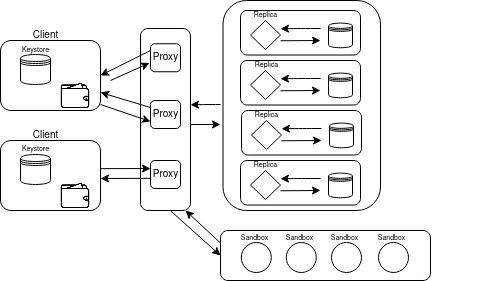
\includegraphics[width=\linewidth]{figures/System_Model.png}
		\caption{BGWS system model.}
	\end{figure}
	
	\subsection{API}
	
	\subsubsection{Register: \textbf{/register/\{who\}}}
	
	Allows a user to be registered in the system. The path parameter \textit{who} is the user's public key, which will be used for future verification of authenticity of messages. The body of the request needs to contain information about the signature and hash algorithms that will be used, as well as information needed for dealing with private operations that will use homomorphic encryption. In case of success, the user will receive a nonce needed for protection against replay attacks in future operations.
	
	\subsubsection{Get Nonce: \textbf{/nonce/\{who\}}}
	
	Allows an already registered user to obtain the shared nonce to request new operations. The path parameter \textit{who} is the user's public key. In case of success, the nonce will be returned to the user.
	
	\subsubsection{Obtain amount: \textbf{/\{who\}/obtainCoins}}
	
	This operation allows a user to add a specified amount to their balance. The path parameter \textit{who} is the user's public key. The request's body contains the amount required signed with the user's private key. In case of success, a new transaction is registered in the system, with the user as the receiver of the amount and \textit{SYSTEM} as the origin. The transaction will be returned to the user with proofs that it was verified and approved by a quorum of replicas. The transaction will be in a pending state, ready to be added in future blocks.
	
	
	\subsubsection{Transfer amount: \textbf{/transferMoney}}
	
	This operation allows a user to transfer money to another user. The body contains a transaction which is signed with the user's private key. If the operation is successful, the user will receive the transaction with proof that it was verified and approved by a quorum of replicas. The transaction will be in a pending state, ready to be added in future blocks.
	
	\subsubsection{Transfer money with privacy: \textbf{/privacyTransfer}}
	Used to register a transaction in the system, where the amount is encrypted with an homomorphic cipher. This allows replicas to perform operations such as obtaining the user's balance with guarantees of privacy regarding the value (only the user can decrypt it). Two different types of transactions can be send. 
	
	In the first case, a transaction is send with the sender being the user who requested the operation. The body of the request contains a transaction with information about who encrypted the amount, and a secret value, which is the amount encrypted with the receiver's public key.
	
	In the second case, the previous transaction needs to have already been registered in the system, otherwise it will not be accepted. In this transaction, the receiver is the user who initiates the request. The amount in this transaction will be encrypted using homomorphic encryption. The value of the amount can be obtained from the secret value of the previous type of transactions (by decrypting with the private key). The transaction also contains the previous transaction's \textit{id} and the remaining fields are equal. 
	
	In either case, the sent information needs to be signed with the user's private key. If it is successful, the transaction will be returned to the user with proofs that it was received, verified and approved by a quorum of replicas. The transaction will be in a pending state, ready to be added in future blocks.

	
	\subsubsection{Obtain private transactions not submitted: \textbf{/\{who\}/obtainNotSubmittedTransactions} }
	
	Allows a user to retrieve the necessary info to submit a private transaction where they are the recipient. The path parameter \textit{who} is the user's public key. In case of success, the user receives a list of information about such transactions.

	\subsubsection{Pick not Mined Transactions: \textbf{/pendingTransactions/\{numPending\}} }
	
	This operation allows a user to obtain transactions not yet mined (transactions that are in a pending state). The number of transactions is specified in the path parameter \textit{numPending}. In case of success, the user will receive a pre-generated block header, of the block containing the requested transactions, which the user can mine.
	
	\subsubsection{Send Mined Block: \textbf{/mine} }
	
	This operation allows a user to send a mined block to be added to the system's blockchain. The request's body contains the mined block and a transaction with a reward for itself. The body's content is signed with the user's private key. In case of success, the new block is added to the system and the transaction reward will be in a pending state, ready to be added in future blocks. The reward transaction is returned to the user with proofs that the operation was accepted and validated by a quorum of replicas.
	
	
	\subsubsection{Ledger of Global Transactions: \textbf{/ledger} }
	
	This operation returns the transactions that are contained in the blockchain. A date interval can be send in the request's body, if the user wants to see transactions created on a certain time period. 
	

	\subsubsection{Ledger of Client transactions: \textbf{\{who\}/ledger} }
	
	This operation returns transactions in the blockchain involving the user. A date interval is sent in the request's body if the user wants to see transactions created on certain time period. The path parameter \textit{who} is the user's public key. The request's body is signed with the user's private key.
	
	\subsubsection{Verify: \textbf{verify/\{id\}} }
	
	This operation returns the blockchain's transaction with the specified id. 
	
	\subsubsection{Obtain last mined block: \textbf{/lastBlock} }
	
	This operation returns the last block that was added to the blockchain.
	
	\subsubsection{Install a Smart Contract: \textbf{/\{who\}/installSmartContract} }
	
	This operation allows the user to install a smart contract in the blockchain. The path parameter \textit{who} is the user's public key. The request's body is signed with the user's private key and contains the byte code of the contract to be installed. If it is successful, the transaction associated with the contract will be returned to the user with proofs that it was received, verified and approved by a quorum of replicas. The transaction will be in a pending state, ready to be added in future blocks.
	
	\subsubsection{Transfer Money With Smart Contract: \textbf{/smartTransfer/\{id\}} }
	
	This operation allows the user to utilize a installed smart contract to transfer money. The path parameter \textit{id} is the id of the smart contract to be used. The request's body is signed with the user's private key and contains the amount to be spent and the destinations. If it is successful, generated transactions will be returned to the user with proofs that they were verified and approved by a quorum of replicas. The transactions will be in a pending state, ready to be added in future blocks.
	
	\subsection{Proxy}
	A proxy is responsible for receiving the REST requests of clients, process the request and re-send the operation to the replicas, or sandboxes, internally. It is also responsible for receiving the replicas and sandboxes replies, and send a response to the client's requests.
	
	\subsection{Replica}
	A replica is responsible to validate requests and execute \textit{read} and \textit{write} operations in the persistent storage. 
	\subsection{Sandbox}
	The sandbox is responsible for loading byte code of new smart contracts, execute it and validate it. 
	
	
	\subsection{Storage Node}
	The storage node contains the persistent data of the system, mainly the ledger and information about the wallets (public key and algorithms associated with the key). Each storage node communicates with a single replica.
	


	\section{Mechanisms and Service Planes}
	In this section we will explain the planes that define the BGWS system and some of its main mechanisms.
	
	\subsection{Service Planes}
	\subsubsection{Consensus Plane}
	The consensus plane unique objective is to solve the agreement between the decision of replicas, about the result of operations, and sandboxes, about the validity of smart contracts. A byzantine fault tolerant consensus algorithm is applied.
	
	\subsubsection{Crypto Services Plane}
	This plane is responsible for all cryptography operations, primitives and for establishing the necessary security protocols. BGWS relies on asymmetric encryption for signatures, partial homomorphic ciphers for privacy transactions and TLS (server-side between proxy/client communication and mutual in proxy/replica, replica/replica, proxy/sandbox and sandbox/sandbox communications).
	
	\subsubsection{Communication Plane}
	The communication plane ensures the use of authenticated perfect links. 
	
	Clients communicate with the system's proxies through the exposed REST API. \textit{Write} operations need to be signed by the clients, contrary to \textit{read} operations. The message flow of \textit{write} and \textit{read} operations will be explained in the following subsection.
	
	Proxies communicate with replicas and sandboxes, sending new requests and receiving their replies.
	
	Replicas are the only components that can communicate with persistent storage nodes. There are no communication links between replicas and sandboxes.
	
	\subsubsection{Block Ordering Plane}
	
	The block ordering plane has the function of validating mined blocks, and therefore, its transactions. If valid, then they can be added to the blockchain.
	
    The mining process consists in a \textit{proof of work}, like that used by Bitcoin. This block is then signed by the user and send to the replicas, via the proxy.
    
    When replicas receive blocks they will verify if the public key is registered in the system. Then, they will check the block's signature. After that, they will verify the validity of proof of work (if the hash satisfies the challenge). Then there will be a check of the integrity of the block's content (if the cumulative hash of the block's content matches the hash of the transactions that it is supposed to contain). Only after passing these validations will the block be proposed as a new block to be added to the chain.
    
    If the \textit{previous hash} field of the block corresponds to the hash of the previous block, the block is added to the blockchain. On the other hand, if it matches with the hash of the block before last one, then the there will be a tiebreaker protocol. If the new block has more transactions or, in case they contain the same transactions, if the \textit{proof of work} is better then the new block is added and the old one removed.
    
    Whenever a new block is added to the blockchain a transaction reward is also inserted into the pending transactions. If a block is replaced, then its corresponding reward transaction is also removed from the pending transactions. 
	
	
	\subsubsection{Sandboxing Plane}
	
	The sandboxing plane has the function of validating new smart contracts. These contracts are executed in a controlled environment, isolated from the main replicas and persistent storage, inside the sandboxes.
	
	To validate a contract, first a temporary snapshot of the system's current state is installed in the sandboxes, then the contract byte code is loaded, and executed while being subject to tests, to determine if it respects the correct policies and does not produce erroneous outputs.
	
	If the contract is valid, then it is redirected to the other replicas to be installed. A smart contract is considered installed after it is contained inside a block in the chain.
	
	\subsubsection{Storage Plane}
	Persistent storage of the ledger is replicated in each storage node of the system. Sandboxes and proxies do not have direct access to this storage.
	
	\subsection{Message flow} 
	In BGWS, the message flow differs if it corresponds to a \textit{write} or a \textit{read} operation in the persistent storage. We will first cover the protocol for most operations, afterwards we will explain the differences involved in the operation to install a smart contract.
	
	\subsubsection{General message flow} 
    The first phase of the protocol is equal to both \textit{read} and \textit{write}, the only difference is that \textit{read} operations do not guarantee order contrary to \textit{write} operations. 	
    
    After a request from a client has been processed by a proxy, it is redirected to the replicas . The request is then processed by the replicas, and the decision is gathered by the proxy. Byzantine consensus is executed and, in the case of \textit{read} operations, the reply is redirected to the client.
    
    For \textit{write} operations, if there was no error found in the request, a second phase of the protocol is executed to commit the value and store it in persistent storage. The \textit{COMMIT} message is sent to the replicas with the value to store. 
    
    Finally the replies are gathered by the proxy and the answer to the request is sent to the client. If there was an error, a protocol to handle the error can be implemented (such as just retrying the request), we did not implement that in the system and assume that the client can just retry the operation.
    
    \subsubsection{Smart contract installation message flow} 
    In the installation of a smart contract, firstly the proxy sends a request to the replicas for a \textit{read} of the system's state. Replicas generate a snapshot of the system, which the proxy send to the sandboxes, to be saved in temporary memory. Only after this first step, does the proxy send the new smart contract byte code to the sandboxes. 
    
    After the validation process of the smart contract, the proxy gathers the decisions of the sandboxes. In case of a valid and safe smart code, the byte code is redirected to the replicas to be installed in the blockchain. 
    
    Finally, in case no other error happened, the protocol proceeds as the last step of the normal message flow.
	
	\section{Implementation}
	
	\subsection{Technology Stack}
	
	The client and the proxy, replica and sandbox components were implemented in Java, as Maven projects. For deployment, we created individual docker images for each component, that were deployed as containers in a custom docker network \textit{bftsmart-net}. Clients were simple java console.
	
	The client and proxy used the Spring Boot framework, due to the simplicity it provided in the establishment of secure communications and specifying different TLS configurations like version, types of authenticity and ciphersuites. 
	
	The proxy, replicas and sandboxes for byzantine consensus, tolerant to non-malicious byzantine faults, used the open source BFT-SMaRt library \cite{bessani2014stateBFTSMART}.
	
	We used Bouncy Castle as the security provider for all non-homomorphic ciphers. For the partial homomorphic primitives, we used the library given by the course professor.
	
	For persistent storage we opted for a NoSQL database, as queries did not need relational dependencies. We used the latest version of Redis key-value stores due to its simple java integration, high performance, easy docker deployment and possibility to configure TLS. 
	
	\subsubsection{Blocks}
	
	The block is compose by a block header and a list of transactions.
	The block header contains the \textit{the previous block hash}, a \textit{timestamp} of the time it was created, the \textit{proof}, which is the random number used in the hash to satisfy the challenge, an \textit{integrity hash} that corresponds to the cumulative hash of all transactions inside the block, a list of the transactions \textit{IDs}, and the \textit{author} of the block.
	
	The \textit{proof} and \textit{author} fields can be modified by the client who mines the block, prior to the generation of the \textit{proof of work}. The mining process occurs only over the \textit{block header}. If the block is approved to enter the block-chain, then the list of transactions is appended to the \textit{block header} forming the final complete \textit{block}.
	
	\subsubsection{Transactions}
	Transactions were designed to be public or private. For this reason, they support multiple fields. 
	Common fields to both types are the \textit{origin}, \textit{destination}, \textit{amount} and \textit{date}, all other fields are \textit{null} in public transactions.
	
	Private transactions also contain a field with the \textit{encrypted amount}, an indication of \textit{who encrypted} it and the \textit{ID} pointing to the original transaction (\textit{null} if it is the original).
	
	As previously said, the pointers to \textit{IDs} and references to \textit{who encrypted} the message are needed in the implementation of private transactions, because they are inserted, in the system, by both the \textit{origin} and \textit{destination}, and need to keep a causal relationship.
	
	Transactions also pass through different verification steps. A transaction becomes a \textit{Signed Transaction} when its signature is approved by the system. At this point it is assigned with an \textit{ID}, and the signature of the request it was proposed in, is associated to it. 
	When a transaction is committed, it becomes a \textit{Valid Transaction}. It contains the hash of the replicas agreed decision, for integrity purposes, and an array with the\textit{IDs} of the replicas who participated in its validation. These extra fields can be used for future auditing.
	
	\subsubsection{Smart Contracts}
	Smart Contracts, are only represented with an interface in the system, but the instances need to follow a specification with fields similar to normal transactions.
	
	The difference to transactions, is that smart contracts are freely programmable and can be referenced by other users to transfer an amount to a set of destinations.
	To do so they have: a \textit{init()} method where the \textit{origin}, \textit{amount} to transfer and set of \textit{destinations} are specified; a \textit{run} method that executes in rounds and produces a set of events; a \textit{readTransaction()} and \textit{readBalance()} methods to read transactions and consult balances (values specified as inputs of the methods); a \textit{getReadTarget()} to specify the \textit{ID} of the next read target in the blockchain, can be a transaction \textit{ID} or a \textit{public key} for balances; a \textit{getOutput()} method to retrieve the final output (set of transactions).
	
    The events produced are the following: \textit{BEGIN}, \textit{READ\_TRANSACTION}, \textit{READ\_BALANCE}, \textit{STOP}. 
    
    The \textit{BEGIN} event happens after a smart contract has been initiated with the necessary and correct info. The \textit{READ\_TRANSACTION} and \textit{READ\_BALANCE} events trigger when the smart contract request a \textit{read} operation of a transaction or balance of a user. The \textit{STOP} event is triggered when the execution terminates and the output is ready to be retrieved.
	
	
	\subsection{Issues}
	\subsubsection{Deployment}
	For ease of deployment of different combinations of proxies, replicas, sandboxes and clients we opted to separate the implementation of each component into a different project. This not only guaranteed separation of concepts, but it also helped with the creation of singular docker images for each component. 
	
	Furthermore, with this separation, the simulation of smart contracts was more realistic as, in the sandbox project, no smart contract class was defined, only an interface. With this, we could verify that the smart contract byte code was actually being dynamically loaded during runtime.
	
	\subsubsection{Container \textit{IPs}}
	The custom docker network \textit{bftsmart-net} was a subnet with IP ranges inside 172.18.0.0/16.
	
    The proxy container for the proxy with \textit{ID} $n$ was named \textit{proxy-$n$} and used the IP 172.18.10.$n$, exposing the port 8443 on 127.0.0.1:900$n$.
    The replica container for the replica with \textit{ID} $n$ was named \textit{replica-$n$} and used the IP 172.18.20.$n$.
    The sandbox container for the sandbox with \textit{ID} $n$ was named \textit{sandbox-$n$} and used the IP 172.18.20.$(2*n)$.
    The storage node containers were redis container. Each storage node of a particular replica with \textit{ID} $n$ was named \textit{redis-$n$}, and used the IP 172.18.30.$n$. 
	
	\subsubsection{Generation of \textit{IDs}}

    In the BGWS system, signed transactions are given a unique \textit{ID}. This \textit{ID} consists in 20 random bytes, generated with a secure random primitive, concatenated to a prefix that depends on the type of transaction. The prefix for normal, block reward, private and smart contracts are, respectively, \textit{0xT}, \textit{0xTB}, \textit{0xTP} and \textit{0xTS}. The prefix and random bytes are separated with a \textit{-}.


	\section{Experimental Evaluation}
	\subsection{Experimental Setup \& Methodology}
	\subsubsection{Validation}
	For validation of new features added to the BGWS system we used a manual client. This was mostly useful for debugging purposes, not for concurrency stress tests.
	
    \subsubsection{Evaluation}
	For evaluation, we created a benchmark client that automated different workloads. This client simply executed the REST requests and saved the time until it received a response from the proxy. The results were saved to different .csv files. We generated plots with a python script.
	
	We run 3 different experiments in a system with the following specifications: AMD Ryzen 7 1700 eight-core processor × 16 CPU and 16GB of RAM DDR4 3200MHz (2 x 8GB).
    On all experiments we used the following constant configurations: TLS version 1.3 with \textit{TLS\_AES\_256\_GCM\_SHA384}; the hash algorithm was \textit{SHA-256} and the mining challenge length was 2bytes (16 leading 0s);  5 benchmark clients with RSA keys of size 3072 bits.

	In the first experiment we studied the overhead associated with tolerating $f$ faults. We simulated 4 different configurations of the system for $f$ equal to 1, 2, 3 and 4 in a running environment with exclusively correct replicas. In these scenarios each client run, concurrently: 50 obtain coins operation; 5 mining operations for blocks containing 10 transactions; 20 requests for the client ledger; 20 requests for the global ledger (both with a time interval that included all transactions since the beginning); 50 transfer money operations; 50 transfer money operations with privacy. 
	
	In the second experiment we studied how the size of blocks influenced the latency of mining operations. We simulated 5 different configurations with block sizes of 10, 20, 30, 40 and 50 transactions with a system tolerating 1 bizantine fault, in a running environment with exclusively correct replicas. The clients run the scenarios sequentially with the following concurrent operations: 50, 100, 150, 200 and 250 obtain coins operations followed by 5 mining operations (accordingly to the compatible block size).
	
	Finally in the last experiment we studied the impact of having one faulty replica in the system. For this experiment we simulated a system configuration tolerant to 1 bizantine fault. In one run we continuously stopped one replica container, for 1s, and restarted it again, for 0.5s. In another run no faults were simulated. Each client executed 500 obtain coins operations for each run.
	
	
	\subsection{Experimental Results}
	
	In this section we present the results as an average of the results for 5 clients running concurrently, and describe the patterns observed.
		
	\begin{figure}[!ht]
		\centering
		\subfloat[REST operations]{
			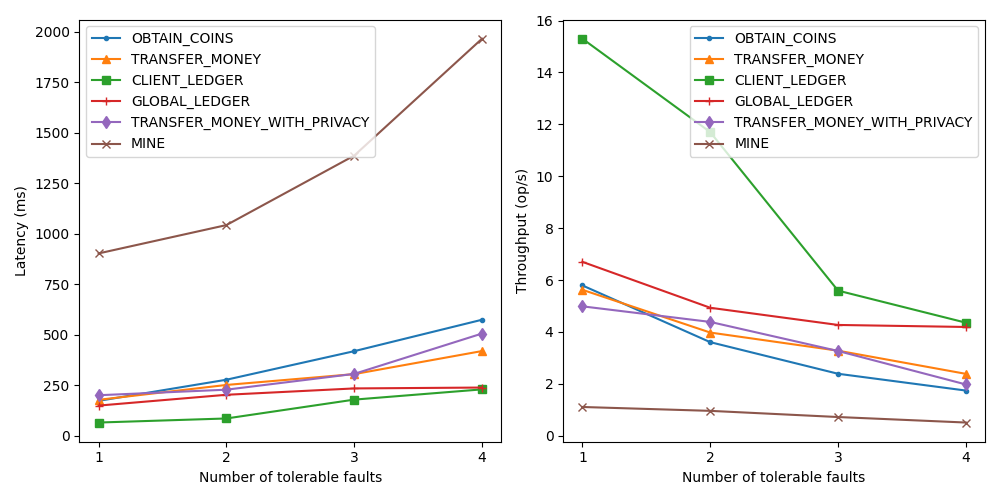
\includegraphics[width=\linewidth]{figures/REST_ops.png}
			\label{REST_ops}
		}
		\vfil
		\centering
		\subfloat[Mining operation]{
			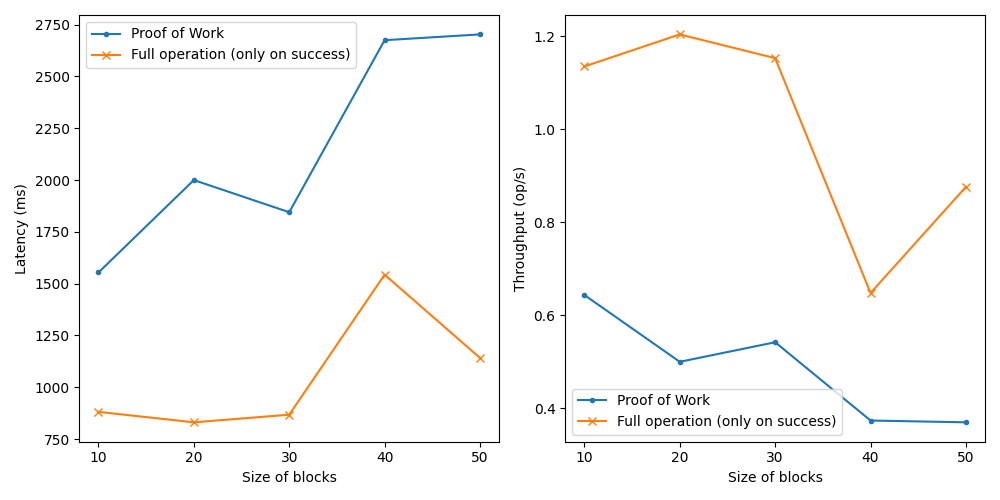
\includegraphics[width=\linewidth]{figures/mining_block.png}
			\label{mining_block}
		}
		\caption{Latency and throughput.}
	\end{figure}
	
	\begin{figure}[!ht]
		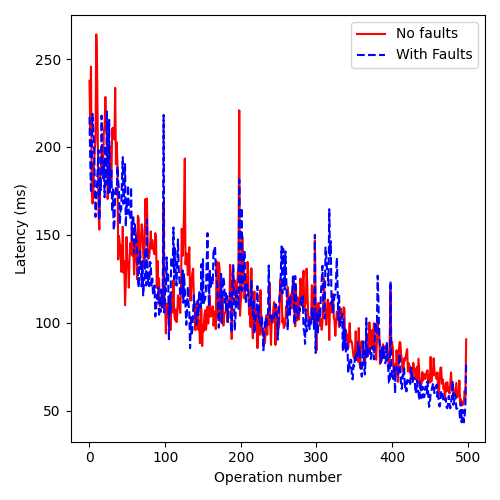
\includegraphics[width=\linewidth]{figures/Fault_Simulations.png}
		\label{Fault simulation}
		\caption{Simulation of run with 1 faulty replica.}
	\end{figure}
	
	In the results of the first experiment \ref{REST_ops} we can observe that the latency increases as the number of bizantine faults, that the system can tolerate, augments. Inversely, the throughput diminishes.

	We can also see that the most costly operation is the mining operation. REST operations that involve \textit{reads} have lower latencies than the ones that involve \textit{writes}.

	From the results of the second experiment \ref{mining_block} we can observe that the duration of the mining operation increases with the block size. Inversely, the throughput diminishes. Furthermore, the latency of successful mine operations is significantly lower than the average of all.

	Finally, the results of the third experiment \ref{Fault simulation} show that the latencies of operations are unaffected in the presence of bizantine faults, within the tolerable interval.
	

	\subsection{Discussion}
	In this section we will discuss the patterns observed in the results of the different experiments.

	For the first experiment, we can explain the increase of latencies (and consequently decrease of throughput) with the overhead of communication between more replicas during the consensus algorithm. Also, the mining operation is the most costly one, due to the computational cost of the challenge.
	Furthermore, the difference in latencies (and throughput) between operations that involve  \textit{reads} and \textit{writes} is explained by the extra communication step in \textit{write} operation.

	In the second experiment, we explain the increase in the duration to compute a \textit{proof of work} with the increase of bytes to hash (more transactions \textit(IDs) in the header, with around 25bytes each). In case of success, we do not observe the trend so easily. There is a certain amount of randomization in the generation of the hashes and, frequently, the fastest to compute the \textit{proof of work} concludes the operation, before the others even send the mined block to be verified by the system. We can conclude that the generation of this proof is the major bottleneck of the operation.

	Finally, in the third experiment no trend can be identified. This concludes that the system is working as expected and, with bizantine faults happening in the tolerable interval, its performance is not affected.
	
	\section{Coverage of Requirements}
	% Coverage of the requirements (Summarize here the coverage (emphasining the completness, correctness, drawbacks, limitations or tradeofs) form the expected requirements.
	
	We covered almost all features required for the final delivery, there is still some work necessary 
	
	\section{Conclusion \& Future Work}

	In this paper we presented the implementation of BGWS, a dependable decentralized ledger for a blockchained global wallet service. We explained its architecture and API, presented and justified the design choices and covered with more detail implementation aspect related with the major components and data structures of the system. 

	We also proposed to study how the number of replicas impact the overall performance of the system, how the size of blocks affects the latency of successful mining operations and how the system tolerates faults.

	Furthermore, we conclude that latencies are higher for operations that involve \textit{writes} and that the most costly operation in the system is the mining operation. Its cost is directly associated with the computational cost of the hash challenge. 

	For future work, we would like to finish the missing feature, like the transactions with smart contracts and evaluate their performance. 

	\ifCLASSOPTIONcaptionsoff
	\newpage
	\fi
	\bibliographystyle{IEEEtran}
	\bibliography{references}
	
\end{document}
